\documentclass[12pt]{article}
 \usepackage[margin=1in]{geometry} 
\usepackage{amsmath,amsthm,amssymb,amsfonts, enumitem, fancyhdr, color, comment, graphicx, environ}
\usepackage{booktabs}
\usepackage{}
\usepackage[colorinlistoftodos]{todonotes}
\usepackage{algorithm}
\usepackage{algpseudocode}
\usepackage{amsmath}
\usepackage{tikz}
\usepackage{subcaption}
\usetikzlibrary{arrows.meta, automata, positioning}


\pagestyle{fancy}
\setlength{\headheight}{65pt}
\newenvironment{problem}[2][Problem]{\begin{trivlist}
\item[\hskip \labelsep {\bfseries #1}\hskip \labelsep {\bfseries #2.}]}{\end{trivlist}}
\newenvironment{sol}
    {\emph{Solution:}
    }
    {
    \qed
    }
\specialcomment{com}{ \color{blue} \textbf{Comment:} }{\color{black}} %for instructor comments while grading
\NewEnviron{probscore}{\marginpar{ \color{blue} \tiny Problem Score: \BODY \color{black} }}

\newcounter{subproblem}
% \renewcommand{\thesubproblem}{\alph{subproblem}} % letters 
\renewcommand{\thesubproblem}{\arabic{subproblem}} % numbers
\newenvironment{subprob}[1][]{
  \refstepcounter{subproblem}
  \begin{trivlist}
  \item[\hskip \labelsep {\bfseries (\thesubproblem)}]
}{
  \end{trivlist}
}
\newenvironment{subsol}
    {\emph{Solution:}
    }
    {
    \qed
    }
%%%%%%%%%%%%%%%%%%%%%%%%%%%%%%%%%%%%%%%%%%%%%%%%%%%%%%%%%%%%%%%%%%%%%%%%%%%%%%%%%
\setlength {\marginparwidth }{2cm}


\newtheorem*{remark}{Remark}

\newcommand{\R}{\mathbb{R}}
\newcommand{\N}{\mathbb{N}}
\newcommand{\Q}{\mathbb{Q}}
\newcommand{\Z}{\mathbb{Z}}
\newcommand{\st}{\text{ s.t }}
\newcommand{\bigO}[1]{\mathcal{O}\left(#1\right)}
\newcommand{\fP}{\mathbb{P}}
\newcommand{\E}{\mathbb{E}}


\usepackage{listings}
\usepackage{xcolor}
\lstset{
  basicstyle=\ttfamily\small,
  backgroundcolor=\color{gray!10},
  frame=single,
  breaklines=true,
  keywordstyle=\color{blue},
  commentstyle=\color{gray},
  stringstyle=\color{red},
  showstringspaces=false,
  numbers=left,            
  numberstyle=\tiny\color{gray}, 
  numbersep=10pt 
}


% titel en auteur van het document
\title{Theory of Algorithms Problem Set \#2}
\author{Nicole Tain}
% \date{} % de datum van het document 

% einde definities; start van de tekst
\begin{document}

\maketitle                  % maakt een kopje met titel, auteur en datum
\thispagestyle{empty}       % zet paginanummering uit voor deze pagina

% kopje met bijbehorende titel; varianten: \subsection, \subsubsection
\section*{Problem 1}
 \begin{center}
    \begin{tikzpicture}[
      mycircle/.style={
         circle,
         draw=black,
         fill=white,
         fill opacity = 0.3,
         text opacity=1,
         inner sep=0pt,
         minimum size=20pt,
         font=\small},
      myarrow/.style={-Stealth},
      node distance=0.6cm and 1.2cm
      ]
      \node[mycircle]  at (-3, 0) (s) {$s$};
      \node[mycircle]  at (-1, 2) (a) {$a$};
      \node[mycircle]  at (1, 2) (b) {$b$};
      \node[mycircle]  at (-1, 0) (c) {$c$};
      \node[mycircle]  at (1, 0) (d) {$d$};
      \node[mycircle]  at (-1, -2) (e) {$e$};
      \node[mycircle]  at (1, -2) (f) {$f$};
      \node[mycircle]  at (3, 0) (t) {$t$};

    \foreach \i/\j/\txt/\p/\pp in {% start node/end node/text/position
      s.45/a.225/4/above/0.5,
      s.00/c.180/9/above/0.5,
      s.315/e.135/14/above/0.5,
      c.90/a.270/4/right/0.5,
      c.270/e.90/4/right/0.5,
      a.00/b.180/4/above/0.5,
      c.00/d.180/11/above/0.5,
      e.00/f.180/5/above/0.5,
      b.225/c.45/1/above/0.5,
      f.135/c.315/3/above/0.5,
      b.270/d.90/15/right/0.5,
      f.90/d.270/4/right/0.5,
      b.315/t.135/16/above/0.5,
      d.00/t.180/5/above/0.5,
      f.45/t.225/6/above/0.5
      }
       \draw [myarrow] (\i) -- node[font=\small,\p,pos=\pp] {\txt} (\j);

    \end{tikzpicture}
    \end{center}
  
\begin{figure}[H]
\centering
\caption{Dijkstra's Aglorithm}
\begin{tabular}{c l c}
\toprule
Curr Node & Dist & Queue \\
\midrule
(start) s & 0 & $\{(l_{s\rightarrow a}, 4), (l_{s\rightarrow c}, 9), (l_{s\rightarrow e}, 14)\}$ \\
s $\rightarrow$ a & 4 & $\{(l_{a\rightarrow b}, 8), (l_{s\rightarrow c}, 9), (l_{s\rightarrow e}, 14)\}$ \\
a $\rightarrow$ b & 8 & $\{(l_{s\rightarrow c}, 9), (l_{b\rightarrow c}, 9), (l_{s\rightarrow e}, 14), (l_{b\rightarrow d}, 23), (l_{b\rightarrow t}, 24)\}$ \\
s $\rightarrow$ c & 9 & $\{(l_{b\rightarrow c}, 9), (l_{c\rightarrow a}, 13), (l_{c\rightarrow e}, 13), (l_{s\rightarrow e}, 14), (l_{c\rightarrow d}, 20), (l_{b\rightarrow d}, 23), (l_{b\rightarrow t}, 24)\}$ \\
b $\rightarrow$ c & 9 & $\{(l_{c\rightarrow a}, 13), (l_{c\rightarrow e}, 13), (l_{s\rightarrow e}, 14), (l_{c\rightarrow d}, 20), (l_{b\rightarrow d}, 23), (l_{b\rightarrow t}, 24)\}$ \\
c $\rightarrow$ a & Found & $\{(l_{c\rightarrow e}, 13), (l_{s\rightarrow e}, 14), (l_{c\rightarrow d}, 20), (l_{b\rightarrow d}, 23), (l_{b\rightarrow t}, 24)\}$ \\
c $\rightarrow$ e & 13 & $\{(l_{s\rightarrow e}, 14), (l_{e\rightarrow f}, 18), (l_{c\rightarrow d}, 20), (l_{b\rightarrow d}, 23), (l_{b\rightarrow t}, 24)\}$ \\
s $\rightarrow$ e & Found & $\{(l_{e\rightarrow f}, 18), (l_{c\rightarrow d}, 20), (l_{b\rightarrow d}, 23), (l_{b\rightarrow t}, 24)\}$ \\
e $\rightarrow$ f & 18 & $\{(l_{c\rightarrow d}, 20), (l_{f\rightarrow c}, 21), (l_{f\rightarrow d}, 22), (l_{b\rightarrow d}, 23), (l_{b\rightarrow t}, 24), (l_{f\rightarrow t}, 24)\}$ \\
c $\rightarrow$ d & 20 & $\{(l_{f\rightarrow c}, 21), (l_{f\rightarrow d}, 22), (l_{b\rightarrow d}, 23), (l_{b\rightarrow t}, 24), (l_{f\rightarrow t}, 24), (l_{d\rightarrow t}, 25)\}$ \\
f $\rightarrow$ c & Found & $\{(l_{f\rightarrow d}, 22), (l_{b\rightarrow d}, 23), (l_{b\rightarrow t}, 24), (l_{f\rightarrow t}, 24), (l_{d\rightarrow t}, 25)\}$ \\
f $\rightarrow$ d & Found & $\{(l_{b\rightarrow d}, 23), (l_{b\rightarrow t}, 24), (l_{f\rightarrow t}, 24), (l_{d\rightarrow t}, 25)\}$ \\
b $\rightarrow$ d & Found & $\{(l_{b\rightarrow t}, 24), (l_{f\rightarrow t}, 24), (l_{d\rightarrow t}, 25)\}$ \\
b $\rightarrow$ t & 24 & $\{(l_{f\rightarrow t}, 24), (l_{d\rightarrow t}, 25)\}$ \\
f $\rightarrow$ t & 24 & $\{(l_{d\rightarrow t}, 25)\}$ \\
\end{tabular}
\end{figure}

The shortest path of distance 24 availble are:
\begin{itemize}
  \item[1)] $s \rightarrow c \rightarrow e \rightarrow f \rightarrow t$
  \item[2)] $s \rightarrow a \rightarrow b \rightarrow c \rightarrow e \rightarrow f \rightarrow t$
  \item[3)] $s \rightarrow a \rightarrow b \rightarrow t$
\end{itemize}




\section*{Problem 2}
\begin{enumerate}
\item [(a)] Let $G$ be a directed graph where each edge $e \in E(G)$ has a length $l_e \geq 0$. Let $s,t \in V(G)$ be vertices of $G$ and let $P$ be a minimum length path from $s$ to $t$ in $G$. If we increase the length of each edge of $G$ by $2$ then $P$ is still a minimum length path from $s$ to $t$ in $G$.
  
  \textbf{False}
  \begin{proof} Take two paths: $P$ and $P'$, with P representing the shortest path from $s \rightarrow t$. $P$ has a distance value of $n$ and contains $k$ edges. $P'$ is some other path with a distance value of $n'$ and contains $k'$ edges. After lengthening each edge, the total distance value of $P$ is $n + 2k$ and the total distance value of $P'$ is $n' + 2k'$. Since these values are arbitrary, it does not matter even though $n < n', ~\exists k, k' \in \Z, \st n' + 2k' < n + 2k$.
  \end{proof}
  
\item [(b)] Let $G$ be a connected undirected graph where each edge $e \in E(G)$ has a length $l_e \geq 0$ and the lengths of the edges of $G$ are all distinct. Let $T$ be the minimum espanning tree of $G$. If we increase the length of each edge of $G$ by $2$ then $T$ is still the minimum spanning tree of $G$.

  \textbf{True}
  \begin{proof} We denote the lengthened graph of $G$ as $G'$. They are essentially the same graph with the same vertices and edges. Therefore any spanning graphs in $G$ are spanning graphs in $G'$ and vice versa. We can denote this relationship using a bijective function: 
    \begin{equation}
    f: G \rightarrow G'; ~f(G(V, E)) = G'(V, E)
    \end{equation}

  Note that any spanning tree by definition is connected and acyclic and therefore has exactly $n-1$ edges. Let $T$ be the minimum spanning tree in $G$ with total length $d$. The total length of $f(T) = d + 2(|V|-1)$. 

  By definition of minimum spanning tree, the total length of any other spanning tree, $G'$, is greater than $d$ due to the distinctness of the edge weights and therefore, the legnth of $f(T') > d + 2(|V|-1)$. 
  
  $f(T)$ is the minimum spanning tree in $G'$.
  \end{proof}


\item [(c)] Let $G$ be a connected undirected graph where each edge $e \in E(G)$ has a length $l_e \geq 0$ and the lengths of the edges of $G$ are all distinct. Let $T$ be the minimum spanning tree of $G$. If $e = \{u,v\} \in E(G)$ is an edge such that $e$ is the longest edge incident to $u$ and $e$ is the longest edge incident to $v$ then $e \notin T$.

\textbf{False}. If $e$ is the only edge that contains either $u$ or $v$, then it must be part of any spanning tree, including the minimum spanning tree $T$.

\item [(d)] Let $G = (V,E)$ and $G' = (V,E')$ be two connected undirected graphs on the same set of vertices $V$ where each edge $e \in E$ has a length $l_e$, each edge $e \in E'$ has a length $l'_e$, and all of these edge lengths are distinct. Let $G''$ be the graph $G'' = (V,E \cup E')$ where edges $e \in E \setminus E'$ have length $l_e$, edges $e \in E' \setminus E$ have length $l'_e$, and edges $e \in E \cap E'$ have length $\min{\{l_e,l'_e\}}$. Letting $T$, $T'$, and $T''$ be the minimum spanning trees of $G$, $G'$, and $G''$ respectively, $T'' \subseteq T \cup T'$ (i.e., every edge in $T''$ is either in $T$ or $T'$).

\textbf{False}
\begin{proof}
  Kruskal's Algorithm for finding minimum subtrees (MST). We claim the MSTs $T, T', T''$ are unqiue due to having distinct edge weights. This is because an MST contains exactly $|V| - 1$ edges and if all edges have different weights, no combonation of $|V| - 1$ edges will amount to the same total weight. Therefore, Kruskal's Algorithm will find the only MST for $G, G', G''$.

  We perform Kruskal's Algorithm on $G, G', G''$. Kruskal's Algorithm takes edges by decending weight and continues or discards them based on if a cycle is formed. In order for an edge, to exist in $T''$ but not in $T' \cup T$, it would need to form a cycle in either $T'$ or $T$ but not in $T''$.

  WLOG, assume that $e_{ab}$ is the first edge which form a cycle in $T$ but not in $T''$. This implies that in $T$, there exists another path, $P$, from $a$ to $b$ which does not exist in $T''$. Let $e_{uv}$ represent some edge in path $P$ which does not exist in $T''$ and $e_{uv}$ would have had to appear earlier in the algorithm. From Kruskal's Algorithm, since $e_{uv}$ is not in $T''$, we know it forms a cycle, which means that there is an alternative path from $u$ to $v$ and therefore, a path from $a$ to $b$. Contradiction.

\end{proof}
\end{enumerate}

\section*{Problem 3a.}
  Sort all intervals $[a_i, b_i]$ lexographically. We will iterativly create a schedule by testing out intervals and confirming if they are the best one. We start with $P_e = 0$ to represent the furthest time covered and an empty schedule. Take the first interval and mark it as a temporary interval, denote as $[a_t, b_t]$.
  
  As we iterate through our list, let $[a_k, b_k]$ represent the next interval:
  \begin{enumerate}
    \item If $a_k \leq P_e$ but $b_k \leq b_t$, then we skip that interval. The temporary interval covers equally as much or more empty slots of time. 
    \item If $a_k \leq P_e$ and $b_k > b_t$, then we replace the temporary interval with $[a_k, b_k]$ becuase $[a_k, b_k]$ covers empty slots of time. 
    \item If $a_k >P_e$, then there exists a gap and $[a_t, b_t]$ is the best possible and furthest reaching interval s.t. $a_t < P_e$. We append this interval to our schedule. $P_e = b_t$ and $[a_k, b_k]$ is now the new temporary interval.
  \end{enumerate}
  
  This process repeats until we either have $P_e \geq T$ or until we reach the end of the list. The last interval will follow the same pattern, except that if it is better than it's precessor, then rather than becomming a temporary interval, it will automatically be added to the schedule.

\section*{Problem 3b.}
We prove the greedy algo stays ahead using the time the $i$-th guard leaves as a measure of progress. We claim that if $S = \{G_1, G_2, \dots, G_m\}$ is the schedule chosen by the greedy algorith. $\forall \text{ valid } S_o = \{G'_1, G'_2, \dots, G'_{m'}\}$, $\forall j \in [m'], \text{ either } m < j \text{ or } b_{i_j} \geq b_{i_j}'$. We prove this by induction.

\begin{proof} We prove this by induction.

  \textbf{Base Case:} $j = 1$. This is trivially true since the greedy algorithm starts at time 0 and looks for the furthest reaching interval s.t. $a_i \leq 0$

  \textbf{Inductive case:} By inductive hypothesis, $\forall 1 \leq j \leq n, \text{ either } m < j \text{ or } b_{i_j} \geq b_{i_j}'$. Consider $j = n + 1$.

  If $n = m$, then $n + 1 > m$. Proof ends trivially.
  
  If $n < m$, then we also know by inductive assumption that $b_{i_n} \geq b_{i_n}'$. Since $S_o$ is a valid schedule, then the next guard in $S_o, ~G_{n+1}' = [a_{i_{n+1}}', b_{i_{n+1}}']$ will have some start time $a_{i_{n+1}}' \leq b_{i_n}' \leq b_{i_n}$ so $G_{n+1}'$ is a valid choice for the next guard in $S$ and $G_{n+1}$ will stay for at least as long as $G_{n+1}'$.

  $\Rightarrow \forall 1 \leq j \leq m', \text{ either } m < j \text{ or } b_{i_j} \geq b_{i_j}'$
\end{proof}

  Therefore, the greedy solution is as optimal as any solution.

\section*{Problem 3c.} Runtime is $O(nlog(n))$. The original sorting is $O(nlog(n))$ and afterwards, we loop through the list, once which is $O(n)$ which doesn't change the asymptotes.

\begin{algorithm}[H]
\caption{Python Implementation}
\begin{lstlisting}
  def schedule(guards: list[list[int]], T: int):
    if T <= 0:
      return 0
    guards.sort()
    P_e = 0
    temp = [0, 0]
    count = 0

    for start, end in guards:
      if end <= temp[1]:
        continue
      
      if start <= P_e:
        temp = [start, end]
        if temp[1] >= T:
            return count + 1
        continue
      else:
        P_e = temp[1]
        count += 1
        if P_e >= T:
          return count
        temp = [start, end]
        
    if P_e < T and temp[1] > P_e:
      P_e = temp[1]
      count += 1

    return count
\end{lstlisting}
\end{algorithm}

\section*{Problem 4: Restaurant Rush (Rephrasing of Problem 13 in Chapter 4 of Kleinberg-Tardos) (20 points)}
You are the owner of a restaurant and there is suddenly a rush of hungry people. Unfortunately, there is currently only one chef in the kitchen so the people are going to have to wait for a while, but you'd like to minimize the total unhappiness.

To model this problem assume that there are $n$ tables. The orders for table $i$ will take time $l_i > 0$ to cook. If their orders come at a time $t_i$, the total unhappiness of table $i$ will be ${u_i}{t_i}$ where $u_i > 0$. Your goal is to minimize the total unhappiness $\sum_{i=1}^{n}{{u_i}{t_i}}$ where 
\[
t_i = l_i + \sum_{j: \text{Table } j \text{ is served before table } i}{l_j}.
\]
\begin{enumerate}
\item[(a)] Serve table with the largest $\frac{u_i}{l_i}$ ratio first and then go down the line, serving those with larger unhappiness coefficents first.
\item[] 
\item[(b)] We prove by exchange. Let $S = \{i_1, i_2, \dots, i_n\}$ be the optimal solution. We aim to show that if $\exists i_k, i_{k+1} \st \frac{u_k}{l_k} < \frac{u_{k+1}}{l_{k+1}}$, then switching the position of these adjacent orders results in a solution as good as $S$.

\begin{equation}
  S' = \{i_1, i_2, \dots, i_{k-1}, i_{k+1}, i_k, \dots, i_n\}
\end{equation}

The only unhappiness values that change are for tables $k$ and $k+1$. We model the change as follows:
\begin{equation}
  \Delta H_k = u_k(\sum_{j = 1}^{j \leq k + 1}l_j - \sum_{j = 1}^{j \leq k}l_j) = u_k(l_{k+1})
\end{equation}

\begin{equation}
  \Delta H_{k+1} = u_{k+1}(l_{k+1} + \sum_{j = 1}^{j < k}l_j - \sum_{j = 1}^{j \leq k+1}l_j) = - u_{k+1}(l_k)
\end{equation}

Therefore the total unhappiness changes by $u_k(l_{k+1}) - u_{k+1}(l_k)$. From the greedy algorithm proposed, we know that $\frac{u_k}{l_k} < \frac{u_{k+1}}{l_{k+1}}$ and so $\Delta H$ is negative. Meaning that the total unhappiness decreases if we switch the position of these tables. The greedy solution is at least as good as the optimal solution $S$.

\item[(c)]Runtime is $O(nlog(n))$. Calculating the ratio is $O(n)$. Sorting by $\frac{u_i}{l_i}$ is $O(nlog(n))$. $O(nlog(n))$ dominates.
\end{enumerate}


\section*{Problem 5: A Pebble Game (20 points)}
Two players are playing the following pebble game. There is a collection of pebbles of different colors. On each of his/her turns, a player takes all of the pebbles of any one color. Each player aims to maximize the number of pebbles they take.
\begin{enumerate}
\item[(a)] At each turn, the player takes the color with the most amount of pebbles.

\item[(b)] Let $S = \{c_1, c_2, \dots, c_n\}$ be the number of pebbles of different colors ordered by magnitude, so $c_i \geq c_j, \forall i < j$. The greedy strategy states that at any turn, you take the color with the great number of pebbles. We denote one round as two turns with both players taking one color.

We claim that the results of each round are

WLOG, assume that one player deviates. At round $i$, the set of remaining pebbles looks like $S = \{c_{i_1}, c_{i_2}, \dots, c_{i_n}\}$. If player 1 deviates and chooses $c_{i_j}$, this  player 2 will choose $c_{i_1}$. This is 

\item[(c)] Let there be 12 pebbles total with the following distributions:
  \begin{enumerate}
    \item[1)] 6 solid purple
    \item[2)] 4 orange / purple
    \item[3)] 6 solid yellow
    \item[4)] 4 orange / yellow
    \item[5)] 1 solid orange
    \item[6)] 1 solid blue
  \end{enumerate}

  If player 1 plays the dominant strategy, the results will be as follows:
\begin{figure}[H]
\centering
\caption{Dijkstra's Aglorithm}
\begin{tabular}{c l c}
\toprule
Curr Node & Dist & Queue \\
\midrule
(start) s & 0 & $\{(l_{s\rightarrow a}, 4), (l_{s\rightarrow c}, 9), (l_{s\rightarrow e}, 14)\}$ \\
s $\rightarrow$ a & 4 & $\{(l_{a\rightarrow b}, 8), (l_{s\rightarrow c}, 9), (l_{s\rightarrow e}, 14)\}$ \\
a $\rightarrow$ b & 8 & $\{(l_{s\rightarrow c}, 9), (l_{b\rightarrow c}, 9), (l_{s\rightarrow e}, 14), (l_{b\rightarrow d}, 23), (l_{b\rightarrow t}, 24)\}$ \\
s $\rightarrow$ c & 9 & $\{(l_{b\rightarrow c}, 9), (l_{c\rightarrow a}, 13), (l_{c\rightarrow e}, 13), (l_{s\rightarrow e}, 14), (l_{c\rightarrow d}, 20), (l_{b\rightarrow d}, 23), (l_{b\rightarrow t}, 24)\}$ \\
b $\rightarrow$ c & 9 & $\{(l_{c\rightarrow a}, 13), (l_{c\rightarrow e}, 13), (l_{s\rightarrow e}, 14), (l_{c\rightarrow d}, 20), (l_{b\rightarrow d}, 23), (l_{b\rightarrow t}, 24)\}$ \\
c $\rightarrow$ a & Found & $\{(l_{c\rightarrow e}, 13), (l_{s\rightarrow e}, 14), (l_{c\rightarrow d}, 20), (l_{b\rightarrow d}, 23), (l_{b\rightarrow t}, 24)\}$ \\
c $\rightarrow$ e & 13 & $\{(l_{s\rightarrow e}, 14), (l_{e\rightarrow f}, 18), (l_{c\rightarrow d}, 20), (l_{b\rightarrow d}, 23), (l_{b\rightarrow t}, 24)\}$ \\
s $\rightarrow$ e & Found & $\{(l_{e\rightarrow f}, 18), (l_{c\rightarrow d}, 20), (l_{b\rightarrow d}, 23), (l_{b\rightarrow t}, 24)\}$ \\
e $\rightarrow$ f & 18 & $\{(l_{c\rightarrow d}, 20), (l_{f\rightarrow c}, 21), (l_{f\rightarrow d}, 22), (l_{b\rightarrow d}, 23), (l_{b\rightarrow t}, 24), (l_{f\rightarrow t}, 24)\}$ \\
c $\rightarrow$ d & 20 & $\{(l_{f\rightarrow c}, 21), (l_{f\rightarrow d}, 22), (l_{b\rightarrow d}, 23), (l_{b\rightarrow t}, 24), (l_{f\rightarrow t}, 24), (l_{d\rightarrow t}, 25)\}$ \\
f $\rightarrow$ c & Found & $\{(l_{f\rightarrow d}, 22), (l_{b\rightarrow d}, 23), (l_{b\rightarrow t}, 24), (l_{f\rightarrow t}, 24), (l_{d\rightarrow t}, 25)\}$ \\
f $\rightarrow$ d & Found & $\{(l_{b\rightarrow d}, 23), (l_{b\rightarrow t}, 24), (l_{f\rightarrow t}, 24), (l_{d\rightarrow t}, 25)\}$ \\
b $\rightarrow$ d & Found & $\{(l_{b\rightarrow t}, 24), (l_{f\rightarrow t}, 24), (l_{d\rightarrow t}, 25)\}$ \\
b $\rightarrow$ t & 24 & $\{(l_{f\rightarrow t}, 24), (l_{d\rightarrow t}, 25)\}$ \\
f $\rightarrow$ t & 24 & $\{(l_{d\rightarrow t}, 25)\}$ \\
\end{tabular}
\end{figure}

\end{enumerate}

\end{document}